\chapter{Notion de fonction et représentation graphique}

\section{Notion de fonction $f(x)$}

\begin{definition}[Fonction]
	Soit $D$ un intervalle ou une réunion d'intervalles de $\R$.

	On définit une \textbf{fonction} $f$ sur $D$ en associant à chaque réel $x$ de $D$ un unique réel noté $f(x)$.
	\begin{enumerate}
		\item $D$ est \textbf{l'ensemble de définition} de $f$.
		\item $x$ s'appelle la \textbf{variable} et $f(x)$ est \textbf{l'image} de $x$ par $f$.
		\item On appelle \textbf{antécédent} de $y$ par $f$ tout réel $x$ de l'ensemble $D$ dont l'image par $f$ est $y$, c'est-à-dire tout réel $x$ de $D$ vérifiant l'égalité $f(x) = y$.
	\end{enumerate}
\end{definition}

\begin{exemple}
	Soit $f$ la fonction définie sur $\R$ par $f(x) = 3x + 1$.
	\bi
	\item L'image d'un réel $x$ par $f$ est le réel $3x + 1$.
	\item La variable peut être une autre lettre que $x$, par exemple $t$. On écrit alors $f(t) = 3t + 1$.
	\ei
\end{exemple}

\begin{remarque}
	Pour traduire le fait qu'à chaque réel $x$ de $D$ on associe un nombre, on utilise aussi la notation : $$f : x \mapsto f(x)$$
\end{remarque}

\begin{definition}
	\textbf{L'ensemble de définition} d'une fonction est le plus grand ensemble des réels qui peuvent avoir une image par cette fonction.

	Cet ensemble de définition peut être imposé par l'énoncé ou par la modélisation. Dans le cas d'une fonction définie par une expression algébrique, l'ensemble de définition est l'ensemble des réels pour lesquels le calcul de l'image est possible :
	\bi
	\item $\pfrac{A}{B}$ est calculable si, et seulement si, $B \neq 0$.
	\item $\sqrt{A}$ est calculable si, et seulement si, $A \ge 0$.
	\ei
\end{definition}

\begin{exemple}
	Soit la fonction $f$ telle que : $$f(x) = \frac{3}{x+1}$$

	Le quotient existe si, et seulement si, $x+1 \neq 0$, c'est-à-dire si, et seulement si, $x \neq -1$.

	La fonction $f$ est donc définie sur $\intoo{-\infty}{-1} \cup \intoo{-1}{+\infty}$.
\end{exemple}

\section{Courbe Représentative d'une Fonction}

\begin{definition}
	Soit $f$ une fonction définie sur un ensemble $D$.

	Dans le plan muni d'un repère, la \textbf{courbe d'équation $y = f(x)$} est l'ensemble des points du plan dont les coordonnées $\coordl{x}{y}$ vérifient la relation $y = f(x)$.

	Cette courbe est appelée \textbf{courbe représentative} ou \textbf{représentation graphique} de la fonction $f$, souvent notée $\Cf$.
\end{definition}

\begin{exemple}
	Soit $f$ la fonction définie sur $D = \intff{-1}{1}$ par $f(x) = x^2 + x$. Sa courbe représentative est l'ensemble des points de coordonnées $\coordl{x}{y}$ tels que $x \in \intff{-1}{1}$ et $y = x^2 + x$.

	Un tableau de valeurs permet d'obtenir les coordonnées des points :
	\[
		A\coordl{-1}{0}, \quad B\coordl{-0{,}5}{-0{,}25}, \quad C\coordl{0}{0}, \quad D\coordl{0{,}5}{0{,}75} \quad \text{et} \quad E\coordl{1}{2}
	\]

	\ms
	\begin{center}
		\begin{tabular}{|c|c|c|c|c|c|}
			\hline
			$x$    & $-1$ & $-0{,}5$  & $0$ & $0{,}5$  & $1$ \\ \hline
			$f(x)$ & $0$  & $-0{,}25$ & $0$ & $0{,}75$ & $2$ \\ \hline
		\end{tabular}
	\end{center}
	\ms

	On place ces points et on les relie par une courbe car il y a une infinité de points lorsque $x$ décrit l'intervalle $\intff{-1}{1}$.

	\begin{center}
		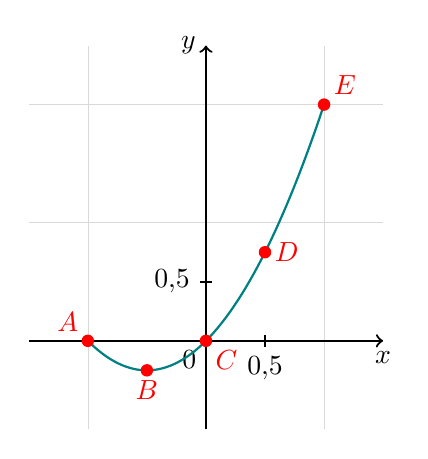
\begin{tikzpicture}[scale=1.5]
			\draw[gray!30,very thin] (-1.5,-0.75) grid (1.5,2.5);
			\draw[->,thick] (-1.5,0) -- (1.5,0) node[below]{$x$};
			\draw[->,thick] (0,-0.75) -- (0,2.5) node[left]{$y$};
			\node[below left] at (0,0) {$0$};
			\draw[thick] (0.5,0.05) -- (0.5,-0.05) node[below]{$0{,}5$};
			\draw[thick] (0.05,0.5) -- (-0.05,0.5) node[left]{$0{,}5$};

			\draw[thick,teal,smooth,samples=100,domain=-1:1] plot (\x,{\x*\x + \x});

			\fill[red] (-1,0) circle (1.5pt) node[above left]{$A$};
			\fill[red] (-0.5,-0.25) circle (1.5pt) node[below]{$B$};
			\fill[red] (0,0) circle (1.5pt) node[below right]{$C$};
			\fill[red] (0.5,0.75) circle (1.5pt) node[right]{$D$};
			\fill[red] (1,2) circle (1.5pt) node[above right]{$E$};
		\end{tikzpicture}
	\end{center}
\end{exemple}

\section{Équations $f(x)=k$ et inéquations $f(x)<k$}

\begin{propriete}
	Soit $f$ une fonction définie sur $D$, de courbe représentative $\Cf$, et $k$ un réel.
	\begin{enumerate}
		\item Les solutions de l'équation $f(x) = k$ sont les abscisses des points d'intersection éventuels de la courbe $\Cf$ avec la droite d'équation $y = k$.
		\item Les solutions de l'inéquation $f(x) < k$ sont les abscisses des points de la courbe $\Cf$ qui sont \og en dessous \fg{} de la droite d'équation $y = k$.
	\end{enumerate}
\end{propriete}

\begin{remarque}
	Pour résoudre l'inéquation $f(x) > k$, on remplace \og en dessous \fg{} par \og au-dessus \fg{} dans la propriété (2).
\end{remarque}

\begin{exemple}
	$f$ est la fonction définie sur $\intff{-1}{3}$ et représentée par la courbe $\Cf$.

	$\Cf$ coupe la droite d'équation $y = 2$ en deux points d'abscisses $1$ et $2$ : ce sont les solutions de l'équation $f(x) = 2$.

	Les solutions de l'inéquation $f(x) < 2$ sont les abscisses des points de $\Cf$ qui sont \og en dessous \fg{} de la droite d'équation $y = 2$.

	L'ensemble solution de $f(x) < 2$ est donc $S = \intfo{-1}{1} \cup \intoo{2}{3}$.

	\begin{center}
		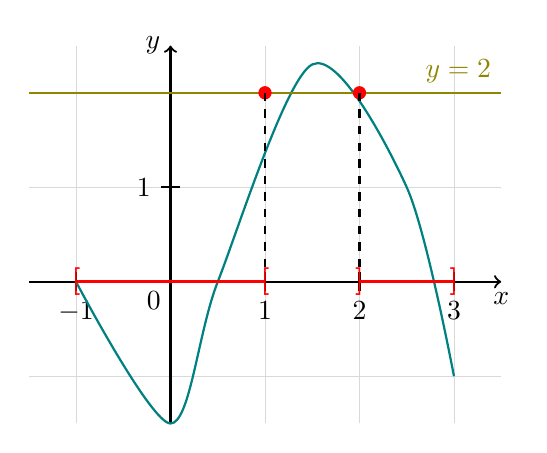
\begin{tikzpicture}[scale=1.2]
			\draw[gray!30,very thin] (-1.5,-1.5) grid (3.5,2.5);
			\draw[->,thick] (-1.5,0) -- (3.5,0) node[below]{$x$};
			\draw[->,thick] (0,-1.5) -- (0,2.5) node[left]{$y$};
			\node[below left] at (0,0) {$0$};

			\draw[thick] (-1,0.1) -- (-1,-0.1) node[below]{$-1$};
			\draw[thick] (1,0.1) -- (1,-0.1) node[below]{$1$};
			\draw[thick] (2,0.1) -- (2,-0.1) node[below]{$2$};
			\draw[thick] (3,0.1) -- (3,-0.1) node[below]{$3$};
			\draw[thick] (0.1,1) -- (-0.1,1) node[left]{$1$};

			% Courbe exemple
			\draw[thick,teal,smooth] plot coordinates {(-1,0) (0,-1.5) (0.5,0) (1.5,2.3) (2.5,1) (3,-1)};
			\node[teal] at (0.2,-0.8) {$\Cf$};

			% Droite y = 2
			\draw[olive,thick] (-1.5,2) -- (3.5,2) node[above left]{$y=2$};
			\fill[red] (1,2) circle (2pt);
			\fill[red] (2,2) circle (2pt);
			\draw[dashed,thick] (1,2) -- (1,0);
			\draw[dashed,thick] (2,2) -- (2,0);

			% Intervalles solutions sur l'axe x
			\draw[red,very thick] (-1,0) -- (1,0);
			\draw[red,very thick] (2,0) -- (3,0);
			\node[red,font=\bfseries] at (-1,0) {$\textbf{[}$};
			\node[red,font=\bfseries] at (1,0) {$\textbf{[}$};
			\node[red,font=\bfseries] at (2,0) {$\textbf{]}$};
			\node[red,font=\bfseries] at (3,0) {$\textbf{]}$};
		\end{tikzpicture}
	\end{center}
\end{exemple}
